\documentclass{article}
\usepackage{amsmath,amsfonts,amsthm,amssymb,amsopn,bm}
\usepackage[margin=.9in]{geometry}
\usepackage{graphicx}
\usepackage{url}
\usepackage[usenames,dvipsnames]{color}
\usepackage{fancyhdr}
\usepackage{multirow}
\usepackage{listings}
\usepackage{hyperref}

\definecolor{keywords}{RGB}{255,0,90}
\definecolor{comments}{RGB}{0,0,113}
\definecolor{red}{RGB}{160,0,0}
\definecolor{green}{RGB}{0,150,0}
 
\lstset{language=Python, 
        basicstyle=\ttfamily\tiny, 
        keywordstyle=\color{keywords},
        commentstyle=\color{comments},
        stringstyle=\color{red},
        showstringspaces=false}

\newcommand{\field}[1]{\mathbb{#1}}
\newcommand{\1}{\mathbf{1}}
\newcommand{\E}{\mathbb{E}} 
\newcommand{\Z}{\mathbb{Z}} 
\renewcommand{\P}{\mathbb{P}}
\newcommand{\R}{\field{R}} % real domain
% \newcommand{\C}{\field{C}} % complex domain
\newcommand{\F}{\field{F}} % functional domain
\newcommand{\T}{^{\textrm T}} % transpose
\def\diag{\text{diag}}

%% operator in linear algebra, functional analysis
\newcommand{\inner}[2]{#1\cdot #2}
\newcommand{\norm}[1]{\left\|#1\right\|}
\newcommand{\twonorm}[1]{\|#1\|_2^2}
% operator in functios, maps such as M: domain1 --> domain 2
\newcommand{\Map}[1]{\mathcal{#1}}
\renewcommand{\theenumi}{\alph{enumi}} 

\newcommand{\Perp}{\perp \! \! \! \perp}

\newcommand\independent{\protect\mathpalette{\protect\independenT}{\perp}}
\def\independenT#1#2{\mathrel{\rlap{$#1#2$}\mkern2mu{#1#2}}}
\newcommand{\vct}[1]{\boldsymbol{#1}} % vector
\newcommand{\mat}[1]{\boldsymbol{#1}} % matrix
\newcommand{\cst}[1]{\mathsf{#1}} % constant
\newcommand{\ProbOpr}[1]{\mathbb{#1}}
\newcommand{\points}[1]{\small\textcolor{magenta}{\emph{[#1 points]}} \normalsize}
\date{{}}

\setlength\parindent{0px}

\begin{document}
\title{Homework \#3}
\author{\normalsize{Winter 2020, STATS 509}\\
\normalsize{Dino Bektesevic}}
\maketitle

\section*{Problem 1}
Let $k > 1$ be a fixed constant. Suppose that $X \sim \hbox{Ber}(1/k)$, so $X$ is a Bernoulli random variable with parameter $1/k$. Let $Y=kX$.
\begin{enumerate}
    \item Find $E(Y)$. First we find what the expectation of $Ber(1/k)$ is:
    
    $$E[X] = 1\cdot P(X=1) + 0\cdot P(X=0) = \frac{1}{k}$$
    Then we can write expectation of Y in terms of X:
    $$E[Y] = E[kX] = k E[X] = k \frac{1}{k} = 1$$.
    Where since $k$ is a constant we can just pull it in front of the expectation. 
    
    \item Find $P(Y \geq k)$; compare this to Markov's inequality.
    
    $$P(Y\geq k) = P(kX \geq k) = P(X\geq 1)$$
    The CDF can only answer "less-than" or "in-range" questions, so we have to rewrite our condition:
    $$P(X\geq 1) = 1 - P(X<1) = 1 - F(1) = 1 - (1 - \frac{1}{k}) = \frac{1}{k}$$
    where we used the Bernouli CDF:
    $$F(x) = \begin{cases} 
	        0 &\mbox{if } x < 0 \\
	        1 - \frac{1}{k} &\mbox{if } 0 \leq x < 1 \\
            1 & \mbox{if } x \geq 1
        \end{cases}  
    $$
    Which is the same expression that is retrieved by Markov/s inequality:
    $$ P(Y\geq k) \leq \frac{E[Y]}{k} = \frac{1}{k}$$
\end{enumerate}


\newpage
\section*{Problem 2}
Suppose that $X$ has the exponential distribution with parameter $\lambda > 0$.
\begin{enumerate}
    \item Find $E(X)$.
    
    \begin{align*}
        E[X] = &\int xf(x,\lambda)dx \\
        & f(x, \lambda) = \begin{cases} 
	            \lambda e^{-\lambda x} &\mbox{if } x \geq 0 \\
	            0 \leq x < 0 &\mbox{if } x < 0
            \end{cases}  \\
        E = &\int_{-\infty}^0 x \cdot 0 dx + \int_0^\infty x \lambda e^{-\lambda x} dx \\
          = &\left[ -\frac{\lambda x + 1}{\lambda} e^{-\lambda x} \right]_0^\infty \\
          = &\frac{1}{\lambda} \left[ -\lambda x e^{-\lambda x} + e^{-\lambda x} \right]_0^\infty
    \end{align*}
    Since it was given that $\lambda>0$, we can see that:
    \begin{align*}
        \lim_{x\rightarrow\infty} x e^{-\lambda x}  = 0 \\
        \lim_{x\rightarrow 0} x e^{-\lambda x}  = 0 \\
        \lim_{x\rightarrow\infty} e^{-\lambda x}  = 1
    \end{align*}
    therefore:
    $$E[X] = \frac{1}{\lambda}$$
    
    \item Find the mode of the distribution of $X$.\par {\it Hint: look at a plot of the pdf.}
    
    The mode is 0 since exponential distribution decreases exponentially for larger than zero, i.e. the PDF will attain its maximum value at 0.
    
    \item Find the CDF $F_X(x)$, and hence the median for $X$. Starting with the CDF
    
    \begin{align*}
        F(x) &= \int_{0}^{x} \lambda e^{-\lambda t} dt \\
            &= -e^{-\lambda t}|_{0}^{x} \\
            &= 1-e^{-\lambda x} \\
    \end{align*}
    noting that integrating for less than zero is just zero. The median is defined as $P(X\leq x) = F(x) = 1/2$. Starting from the CDF we just calculated:
    \begin{align*}
        \frac{1}{2} &= 1 - e^{-\lambda x} \\
        e^{-\lambda x} &= \frac{1}{2} \\
        -\lambda{x} &= \ln\frac{1}{2} = \ln1 - \ln2 \\
        x &= \frac{\ln2}{\lambda}
    \end{align*}
    
    \newpage
    \item Show that $E(X) = \int_0^\infty (1-F_X(x)) dx.$
    \begin{align*}
        E[X] &= \int_0^\infty 1-F(x) dx \\
        &= \int_0^\infty e^{-\lambda x} dx \\
        &= \frac{e^{-\lambda x}}{\lambda} \bigg|_0^\infty \\
        &=\frac{1}{\lambda}
    \end{align*}
\end{enumerate}	
	


\newpage
\section*{Problem 3}
Suppose that $X$ is a continuous random variable, which is always positive, so that $P(X> 0)=1$.
Show that in this case the relationship given in Qu.~2(d) still holds (in other words, without assuming $X$ has
an exponential distribution).\par
{\it Hint: Replace $F_X$ in the expression above with the integral of the pdf (remember not to use $x$ as the name of the dummy variable `$d$blah' in your integral). This gives you a double integral. Now reverse the order in which you do the two integrals. It will help to draw a picture of the region you are integrating over.}

By definition:
$$ F(x) = P(X\leq x) = 1 - P(X>x) = 1 - \int_x^\infty f(t) dt$$
So that
\begin{align*}
    E[X] &=  \int_0^\infty xf(x) dx \\
    &=\int_0^\infty 1- \left(1 - \int_x^\infty f(t) dt\right) dx \\
    &= \int_0^\infty\int_x^\infty f(t) dtdx 
\end{align*}

If we want to follow the hint and perform the integration over x first, with the current problem setup it is obvious that we would not be logically consistent if we did not address the integration limits. Because of how we set up the variables in the CDF definition we can see that $t\geq x$ and from the problem set up we know that $x\geq 0$ we can say that $0\leq x \leq t$.
\begin{center}
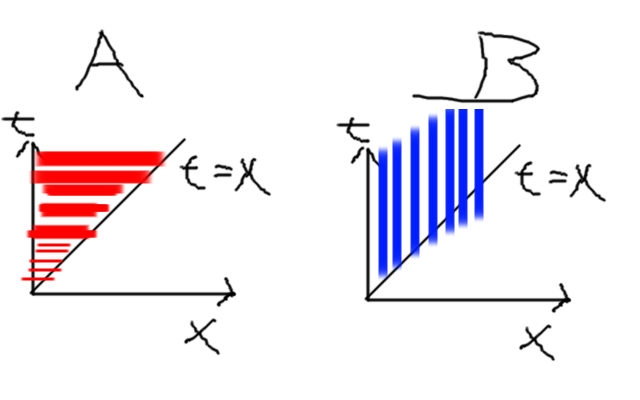
\includegraphics[width=200px]{STATS509/HW3/picasso2.png}
\end{center}
In effect, instead of going from 0 to infinity, adding up all of f(t)'s for each x to infinity as we go along, we are going from 0 to infinity in t, but adding up all individual x's from 0 to t. 
\begin{align*}
    E[X] &=  \int_0^\infty\int_x^\infty f(t) dtdx  =  \int_0^\infty\int_0^t f(t) dxdt  \\
    &= \int_0^\infty \left[xf(t)\right]\big|_0^t dt \\
    &= \int_0^\infty tf(t) dt 
\end{align*}
Which is exactly the definition of the expectation value we started from, except with a differently named dummy variable.


	
\newpage
\section*{Problem 4}
This question aims to make concrete the moment generating function via simulation in {\tt R}: ({\it Note: this is a computational exercise; almost no theoretical work is required.})
\begin{enumerate}
    \item Simulate $1000$ values from $X \sim {\cal N}(5,1)$ distribution, that is, the Normal Distribution with mean $5$, variance $1$.
    
    \lstinputlisting[linerange={0-3,5-5}]{HW3Code/problem4.py}
    
    
    \item Let $V = e^{0.01 X}$. Using your simulations from (a), obtain $1000$ simulations from $V$. Using your simulations find approximately $E(V) = E(e^{0.01 X})$. {\it Hint: Both of these steps are very easy in {\tt R}.}
    
    \lstinputlisting[linerange={9-10}]{HW3Code/problem4.py}
    \lstinline[language=Python]{>>> Empirical expectation value is 1.0513345653017423}
    
    \item Let $W = e^{-0.01 X}$. Using your simulations from (a), obtain $1000$ simulations from $W$. Using your simulations find approximately $E(W) = E(e^{-0.01 X})$.
    
    \lstinputlisting[linerange={14-15}]{HW3Code/problem4.py}
     \lstinline[language=Python]{>>> Empirical expectation value is 0.9514016522849649}
    
    \item Using your answers to (b) and (c), find $ \left. \frac{\partial}{\partial t} E(e^{tX}) \right|_{t=0}$ approximately. Is this what you expect? Explain.\par
    {\it Hint:  $$ \left. \frac{\partial}{\partial t} E(e^{tX}) \right|_{t=0}\;\; \approx\;\; \frac{ E(e^{\delta X}) - E(e^{-\delta X})}{2\delta},$$ for small $\delta$.}
        
        \lstinputlisting[linerange={19-20}]{HW3Code/problem4.py}
         \lstinline[language=Python]{>>> Empirical expectation value is 5.003428743342296}
         
         I expected this. A thousand samples is large enough to be close to the truth, given no errors were made in code. Mathematically, we expand into series the term:
         $$E(e^{\delta X}) = 1 + \delta E(X) + ... $$
         keeping just the first two terms we can substitute them into the expression for derivative approximation:
         \begin{align*}
          \left. \frac{\partial}{\partial t} E(e^{tX}) \right|_{t=0}\;\; &\approx\;\; \frac{ E(e^{\delta X}) - E(e^{-\delta X})}{2\delta} \\
            &= \frac{1 + \delta E(X)  - (1 - \delta E(X))}{2\delta} \\
            &= \frac{2\delta E[X]}{2\delta} = E[X] = 5
        \end{align*}
         when $\delta<<1$.
         
\end{enumerate}


\newpage
\section*{Problem 5}
A random variable $X$ with support on $\mathbb{R}$ has pdf 
$$ f_X(x) = e^{-c|x|}$$
where $c >0$ is a fixed constant.
\begin{enumerate}

    \item Find $c$.
    
    From normalization condition, applying symmetry, we have:
    \begin{align*}
      1 &= \int_{-\infty}^\infty e^{-c|x|}dx \\
      &= 2\int_{0}^\infty e^{-cx}dx  \\
      &= \frac{2}{c} (-e^{-cx})\big|_0^\infty = \frac{2}{c} (-0+1) \\
      &= \frac{2}{c} \\
      c &= 2
    \end{align*}    

    \item Find the mgf $M_X(t) = E[e^{tX}]$ for $X$. {\it Hint: It may be helpful to split the integral into two pieces.}
    
    \begin{align*}
      M_X(t) &= E[e^{tX}] = \int e^{tx} e^{-c|x|} dx  \\
      &= \int_{-\infty}^0 e^{tx} e^{cx} dx + \int_{0}^\infty e^{tx} e^{-cx} dx  \\
      &= \int_{-\infty}^0 e^{(t+2)x} dx + \int_{0}^\infty e^{(t-2)x} dx  \\
      &= \frac{e^{(t+2)x}}{t+2}\bigg|_{-\infty}^0 + \frac{e^{(t-2)x}}{t-2}\bigg|_0^{\infty}  \\
      &= \frac{1}{t+2} \left[ 1 - \lim_{x\rightarrow -\infty} e^{(t+2)x} \right]  +  \frac{1}{t-2} \left[ \lim_{x\rightarrow \infty} e^{(t-2)x} - 1 \right]  \\
    \end{align*}    
    
    \item  State the range of values of $t$ for which $M_X(t)$ is defined. In other words, the range of values of $t$ for which $E[e^{tX}] < \infty$.
    
    Moment generating function will be undefined when $t+2<0$ because term $\lim_{x\rightarrow -\infty} e^{(t+2)x} \rightarrow \infty$ diverges, i.e. $e^\infty$. The expression will also be undefined for $t-2>0$ again because $\lim_{x\rightarrow \infty} e^{(t-2)x} \rightarrow \infty$ term diverges, i.e. $e^\infty$ again. Moreover for $t\in \{-2, 2\}$. the MGF is yet again undefined due to factors $(t\pm 2)^{-1}$. So only for $-2<t<2$ do we have an usable expression: 
    $$M_X(t) = \frac{1}{t+2}  -  \frac{1}{t-2} = \frac{-4}{t^2-4} $$
    
    \newpage
    \item Using your answer to (b), or otherwise, find $E[X]$, $E[X^2]$ and $V(X)$.
    \begin{align*}
        M'(t)  &= \frac{-1}{(t+2)^2} + \frac{1}{(2-t)^2} \\
        M''(t) &= \frac{2}{(t+2)^3} + \frac{2}{(2-t)^3} \\
    \end{align*}
    And we know that the following relationships hold:
    \begin{align*}
        E[X] &= M'(0) = 0\\
        E[X^2] &= M''(0) = \frac{1}{2}\\
        V[X] &= E[X^2] - E[X]^2 = \frac{1}{2} \\
    \end{align*}
\end{enumerate}



\newpage
\section*{Problem 6}
Suppose that $X$ and $Y$ are random variables, and $Y = a + bX$.  
Find an expression for the mgf for $Y$, $M_Y(t)$ in terms of the mgf for $X$, $M_X(t)$.

    \begin{align*}
        M_Y(t) &= E\left[e^{tY}\right] = E\left[e^{t(a+bX)}\right]\\
        &= E\left[e^{ta+tbX}\right] = E\left[e^{ta}e^{tbX}\right] \\
        &= e^{ta} E\left[e^{tbX}\right] \\
        &= e^{ta} M_X(tb) \\
    \end{align*}
    
    
    

\newpage
\section*{Problem 7}
Let $X$ be a random variable with mgf $M_X(t)$. For $t >0$ define the random variables $Z_t = e^{tX}$.\par 
(Here we are defining a set of random variables, one for each value of $t$.)
\begin{enumerate}
    \item Find a relation between $P(X \geq a)$ and $P(Z_t \geq e^{ta})$. 
    
    \begin{align*}
        P(Z_t \geq e^{ta}) &= P(e^{tX} \geq e^{ta}) \\
        &= P(tX \geq ta) \\
        &= P(X \geq a)
    \end{align*}
    Because $\ln$ is a nice function and $t>0$. 
    
    \item By using the result from (a) and applying Markov's inequality find an upper bound on {\color{blue} $P(X \geq a)$} in terms of $M_X(t)$. 
    
    \begin{align*}
        P(X \geq a) &\leq \frac{E[X]}{a} \\
        P(e^{tX} \geq e^{ta}) &\leq \frac{E[e^{tX}]}{e^{ta}} \\
        P(Z_t \geq e^{ta}) &\leq \frac{M_X(t)}{e^{ta}} \\
        P(X \geq a) &\leq \frac{M_X(t)}{e^{ta}} \\
    \end{align*}
    Where we used a) in the last line of the problem. 
    
    \item Now suppose that $X$ is a Poisson distribution with parameter  $\lambda$. Use Markov's inequality, as given in the Lecture 4, Slide 4 to obtain an upper bound on $P(X \geq k\lambda)$ where $k> 0$.
    
    \begin{align*}
        P(X \geq k\lambda) &\leq \frac{E[X]}{k\lambda} \\
        &\leq \frac{\lambda}{k\lambda} = \frac{1}{k}
    \end{align*}
    
\end{enumerate}

Since $X$ is a Poisson random variable $M_X(t) = \exp\left[\lambda(e^t - 1)\right]$. 

\begin{itemize}
    \item[d.] Use the result in (b) to find an upper bound on $P(X \geq k\lambda)$, for $k\geq 1$, in terms of $t$, $k$ and $\lambda$.
    \begin{align*}
        P(X \geq k\lambda ) &\leq \frac{M_X(t)}{e^{tk\lambda}} \\
        &\leq e^{-tk\lambda} e^{\lambda(e^t-1)} \\
        &\leq e^{\lambda e^t-(1+tk)\lambda} = e^{\lambda e^t}e^{-\lambda kt}e^{-1}
    \end{align*}
    
    \newpage
    \item[e.] By differentiating your answer to {\color{blue}(d)} with respect to $t$, find the value of $t$ that gives the tightest upper bound on $P(X \geq k\lambda)$, and state this upper bound.
    
    \begin{align*}
        \frac{\partial}{\partial t} e^{\lambda e^t}e^{-\lambda kt}e^{-1} &= 0 \\
        e^{\lambda e^t - \lambda k t - 1}(\lambda e^t - \lambda k) &= 0 \\
        \frac{e^{\lambda e^t}e^{-\lambda kt}}{e} \lambda (e^t - k) &= 0 \\
        e^{\lambda e^t}e^{-\lambda kt} (e^t - k) &= 0 \\
        \rightarrow (e^t - k)  \rightarrow t &= \ln k
    \end{align*}
    Technically we should be looking at the second derivative to confirm this is a maximum or minimum but I think it's safe to assume the extrema is an upper bound on $P(X \geq k\lambda)$:
    \begin{align*}
        P(X \geq k\lambda) &\leq e^{\lambda e^{\ln k}}e^{-\lambda k\ln k}e^{-1} \\
        &\leq \frac{e^{\lambda k}e^{-\lambda k\ln k}}{e} = \frac{e^{\lambda k(1-\ln k)}}{e}
    \end{align*}
    
    \item[f.] Let $\lambda=2$ and $k=3$, compute the upper bound from (c), the upper bound from (e) and by using {\tt ppois} in {\tt R}, find the exact probability $P(X \geq k\lambda)$.\par
    {\it Hint: when computing the exact probability be careful to include the probability that $P(X=6)$.}
    
    Note that to compute $P(X \geq k\lambda) = 1 - P(x<k\lambda) = 1 - F(k\lambda)$ where F is the CDF but I accidentally already overloaded capital letters.
    
    \lstinputlisting{HW3Code/problem7f.py}
    \lstinline[language=Python]{>>> Upper bound as estimated in problem c: 0.3333333333333333} \newline
    \lstinline[language=Python]{>>> Upper bound as estimated in problem E: 0.20358458038762214} \newline
    \lstinline[language=Python]{>>> Upper limit as evaluated via CDF: 0.1847367554762278}\newline

\end{itemize}



\newpage
\section*{Problem 8}
Let $X$ be a standard normal random variable.
\begin{enumerate}
    \item Find the mgf for $X$;\\
    {\it As always, remember to specify the values of $t$ for which it is defined.}
    
    The standard definition of the PDF of a normal distribution is:
    $$ N(0,1) = f(x) = \frac{1}{\sqrt{2\pi}} e^{-\frac{x^2}{2}} $$
    So by the definition of an MGF:
    \begin{align*}
        M(t) &= \int_{-\infty}^\infty e^{tx} \frac{1}{2\pi} e^{-\frac{x^2}{2}} dx \\
        M(t) &=  \frac{1}{\sqrt{2\pi}} \int_{-\infty}^\infty e^{tx-\frac{x^2}{2}} dx \\
        M(t) &=  \frac{1}{\sqrt{2\pi}} \int_{-\infty}^\infty e^{\frac{1}{2}(-x^2 + 2tx - t^2 + t^2)} dx \\
        M(t) &=  \frac{1}{\sqrt{2\pi}} \int_{-\infty}^\infty e^{-\frac{1}{2}(x^2 - 2tx + t^2 - t^2)} dx \\
        M(t) &=  \frac{1}{\sqrt{2\pi}} \int_{-\infty}^\infty e^{-\frac{1}{2}((x-t)^2 - t^2)} dx \\
        M(t) &=  \frac{1}{\sqrt{2\pi}} \int_{-\infty}^\infty e^{-\frac{1}{2}(x-t)^2 + \frac{t^2}{2}} dx \\
        M(t) &=  \frac{1}{\sqrt{2\pi}} \int_{-\infty}^\infty e^{-\frac{1}{2}(x-t)^2} e^{\frac{t^2}{2}} dx \\
        M(t) &=  \frac{e^{\frac{t^2}{2}}}{\sqrt{2\pi}} \int_{-\infty}^\infty e^{-\frac{1}{2}(x-t)^2} dx \\
        & u = x - t \rightarrow du = dx \\
        M(t) &=  \frac{e^{\frac{t^2}{2}}}{\sqrt{2\pi}} \int_{-\infty}^\infty e^{-\frac{u^2}{2}} du \\
        M(t) &=  \frac{e^{\frac{t^2}{2}}}{\sqrt{2\pi}} \sqrt{2\pi} \\
        M(t) &=  e^{\frac{t^2}{2}} \\
    \end{align*}

    \newpage
    \item Use (a) to find $E(X)$, $E(X^2)$, $V(X)$ and $E(X^3)$.
    
    Following the definitions for expectation value:
    \begin{align*}
        E[X] &=  M'(0) \\
        &=  te^{\frac{t^2}{2}}\bigg|_{t=0} \\
        &= 0
    \end{align*}
    for expectation of:
    \begin{align*}
        E[X^2] &=  M''(0) \\
        &= \frac{\partial}{\partial t} \left( te^{\frac{t^2}{2}} \right) \\
        &= \left[ t^2e^{\frac{t^2}{2}} +  e^{\frac{t^2}{2}} \right] \bigg|_{t=0} \\
        &= 1
    \end{align*}
    for expectation of: 
    \begin{align*}
        E[X^3] &=  M'''(0) \\
        &= \frac{\partial^2}{\partial t^2} \left( te^{\frac{t^2}{2}} \right) \\
        &= \frac{\partial}{\partial t} \left( t^2e^{\frac{t^2}{2}} +  e^{\frac{t^2}{2}} \right)\\
        &= \left[ t^3e^{\frac{t^2}{2}} + 2te^{\frac{t^2}{2}} +  te^{\frac{t^2}{2}} \right] \bigg|_{t=0} \\
        &= 0
    \end{align*}
    for variance:
    \begin{align*}
        V[X] &= E[X^2] - E[X]^2 \\
        &= 1
    \end{align*}
    
\end{enumerate}


\end{document}
